\label{sec:vbf-parsigz}

We parameterize the signal and \zjets{} Monte Carlo templates to smooth out the local fluctuations coming from the limited statistics using a histogrammed Bukin function. The MC templates and parametrization of signal and \zjets{} \Mbb{} distributions are shown in Figures~\ref{fig:vbf-sigpar_alt} and \ref{fig:vbf-zpar_alt}. The $\chi^2$ between simulated and fitted distributions are summarized in Table~\ref{tab:sigpar_alt}. In general, the $\Mbb$ distributions for the Higgs signal and \zjets{} are well represented by the Bukin function. The potential bias of using smoothed MC templates is studied in the full profile likelihood fit. Perfect closure is obtained with $\mu_{H}=1$ and $\mu_{Z}=1$, as injected in the Asimov data.  Therefore we conclude that the parameterized templates produce no significant bias.  The likelihood fit is described in detail later in this section.

\begin{table}[htbp]
\centering
\begin{tabular}{|c|c|c|c|c|}
\hline
\multicolumn{5}{|c|}{$H\rightarrow b\bar b$ \fourcentral}                                                    \\ \hline
Region                                & \multicolumn{2}{c|}{SR I}        & \multicolumn{2}{c|}{SR II}        \\ \hline
\multicolumn{1}{|l|}{$\chi^2$ (Prob)} & \multicolumn{2}{c|}{0.85(0.64)}  & \multicolumn{2}{c|}{1.01(0.44)}   \\ \hline
\multicolumn{5}{|c|}{$H\rightarrow b\bar b$ \twocentral}                                                   \\ \hline
Region                                & SR I            & SR II          & SR III           & SR IV          \\ \hline
\multicolumn{1}{|l|}{$\chi^2$ (Prob)} & 1.06 (0.39)     & 0.77 (0.71)    & 1.10 (0.35)      & 1.21 (0.25)    \\ \hline
\multicolumn{5}{|c|}{\zjets}                                                                                 \\ \hline
Channel                               & \multicolumn{2}{c|}{\twocentral} & \multicolumn{2}{c|}{\fourcentral} \\ \hline
\multicolumn{1}{|l|}{$\chi^2$ (Prob)} & \multicolumn{2}{c|}{1.7 (0.04)}  & \multicolumn{2}{c|}{1.32 (0.17)}  \\ \hline
\end{tabular}
\caption{Goodness of fit for the Bukin parameterizations and signal and \zjets{} \Mbb{} distributions. There are not enough events for the \zjets{} sample to divide amongst BDT regions, therefore a the goodness of fit is shown for each channel preselection.}
\label{tab:sigpar_alt}
\end{table}

\begin{figure}[htbp]
  \centering    
 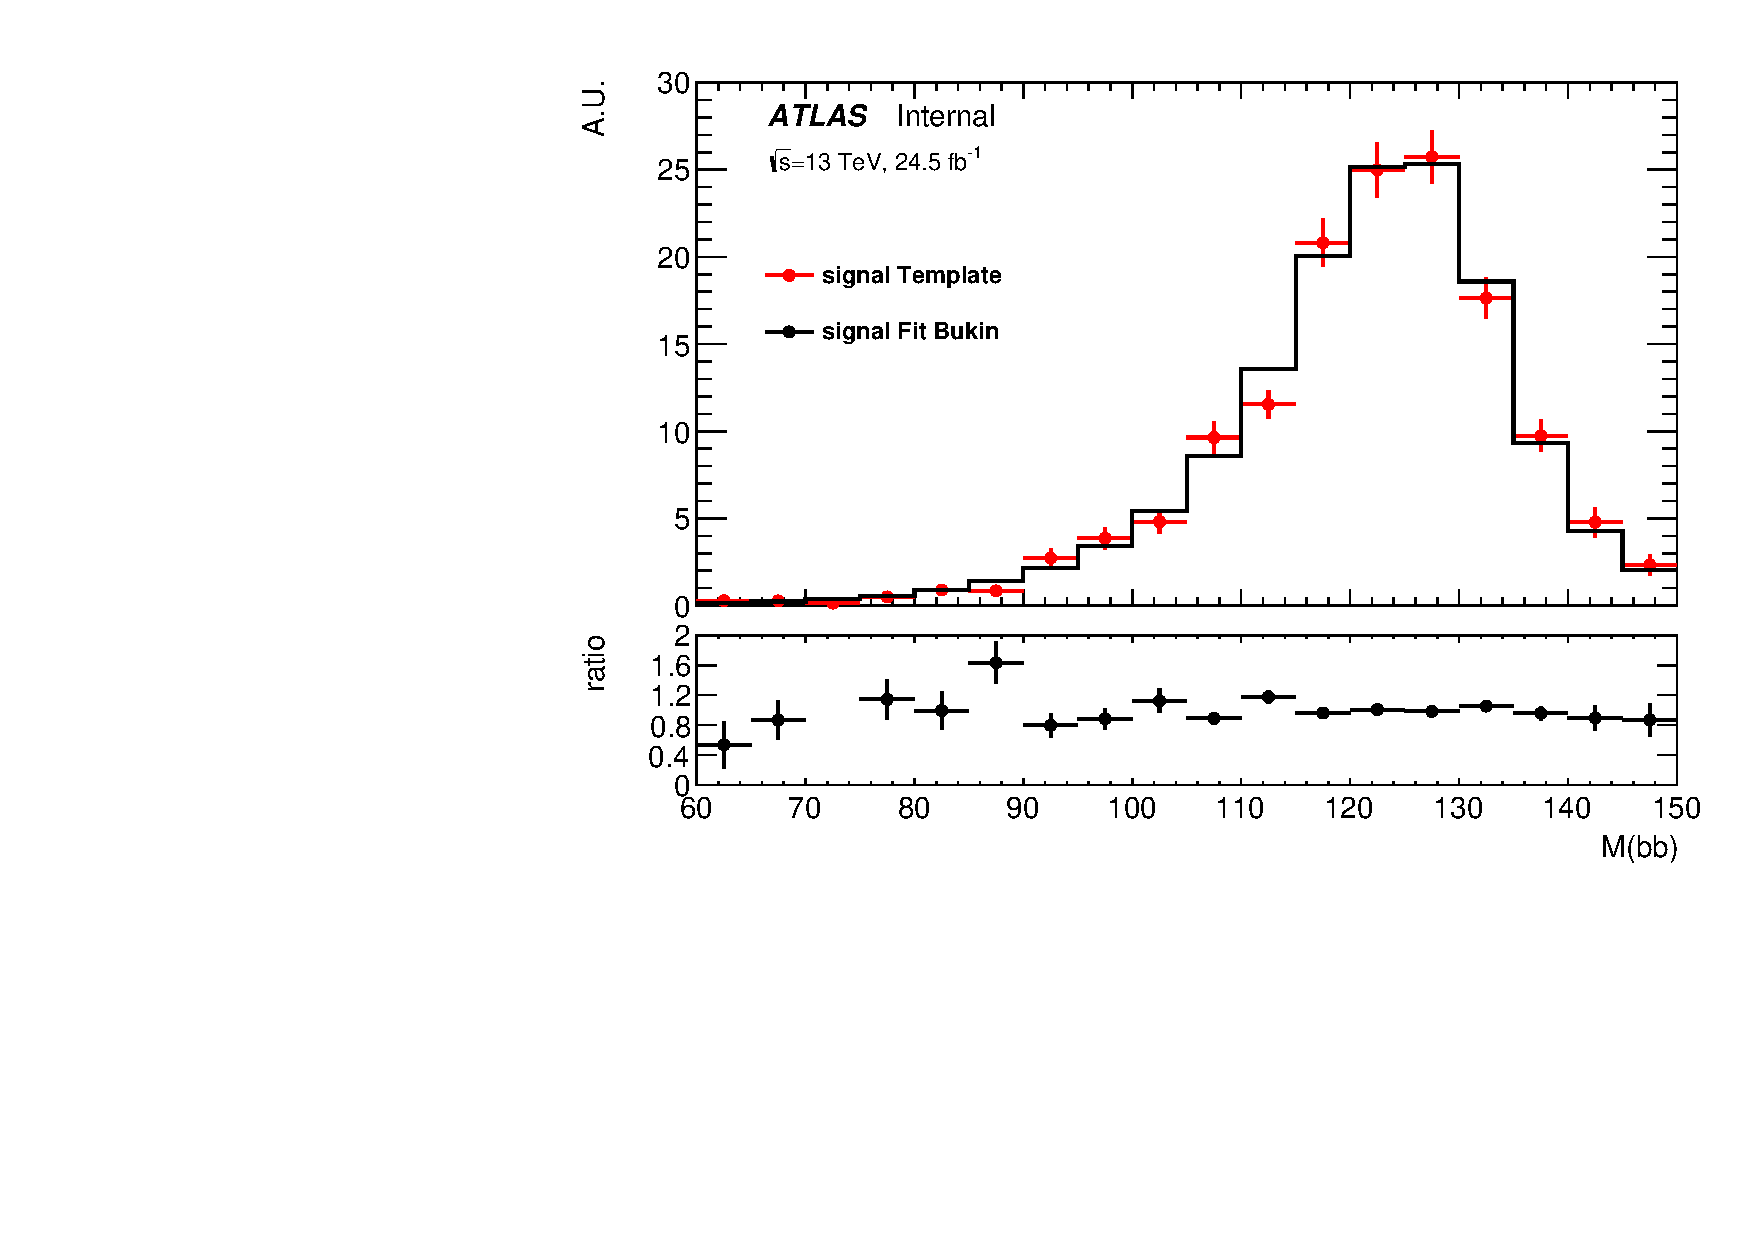
\includegraphics[width=0.45\textwidth]{figures/VBF/sig_2cen_SRI.pdf}
% 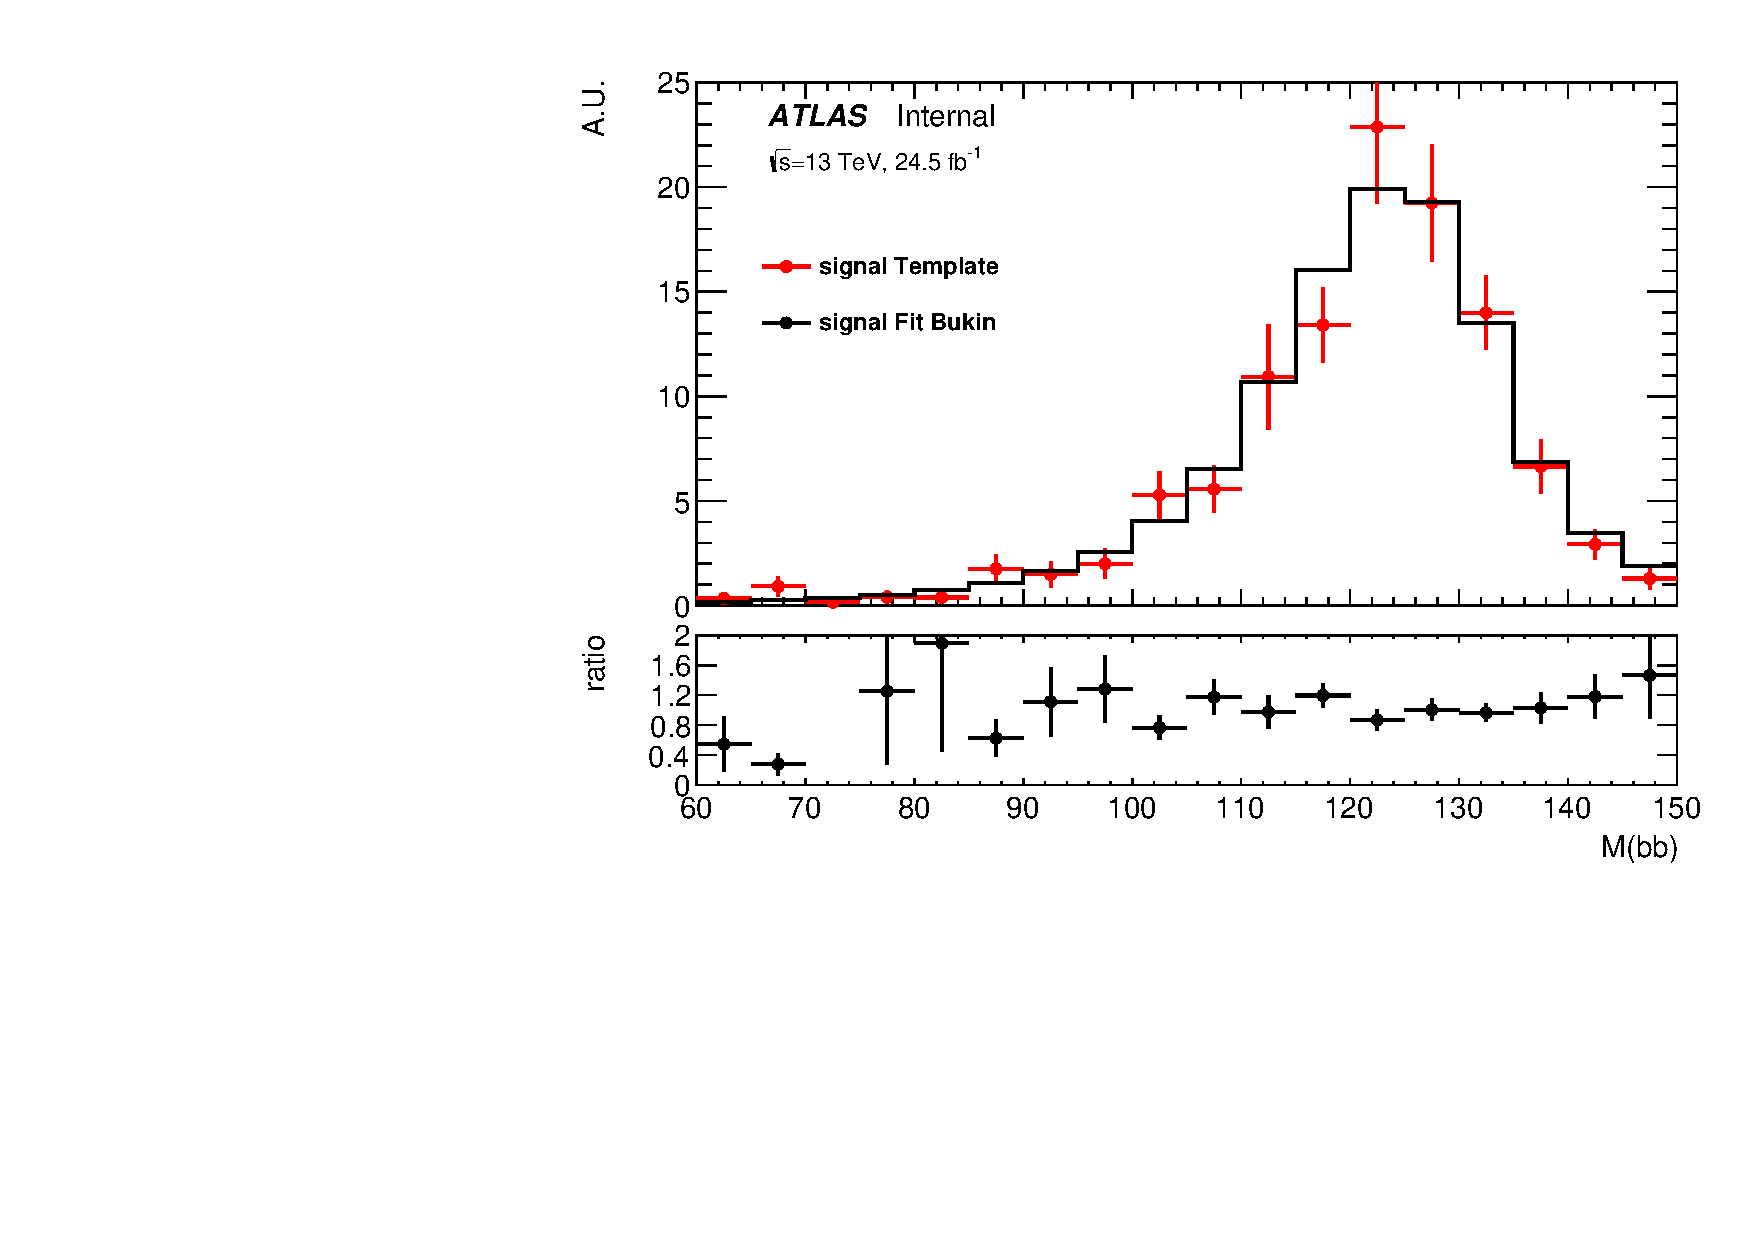
\includegraphics[width=0.24\textwidth]{figures/VBF/sig_2cen_SRII.pdf}\\
 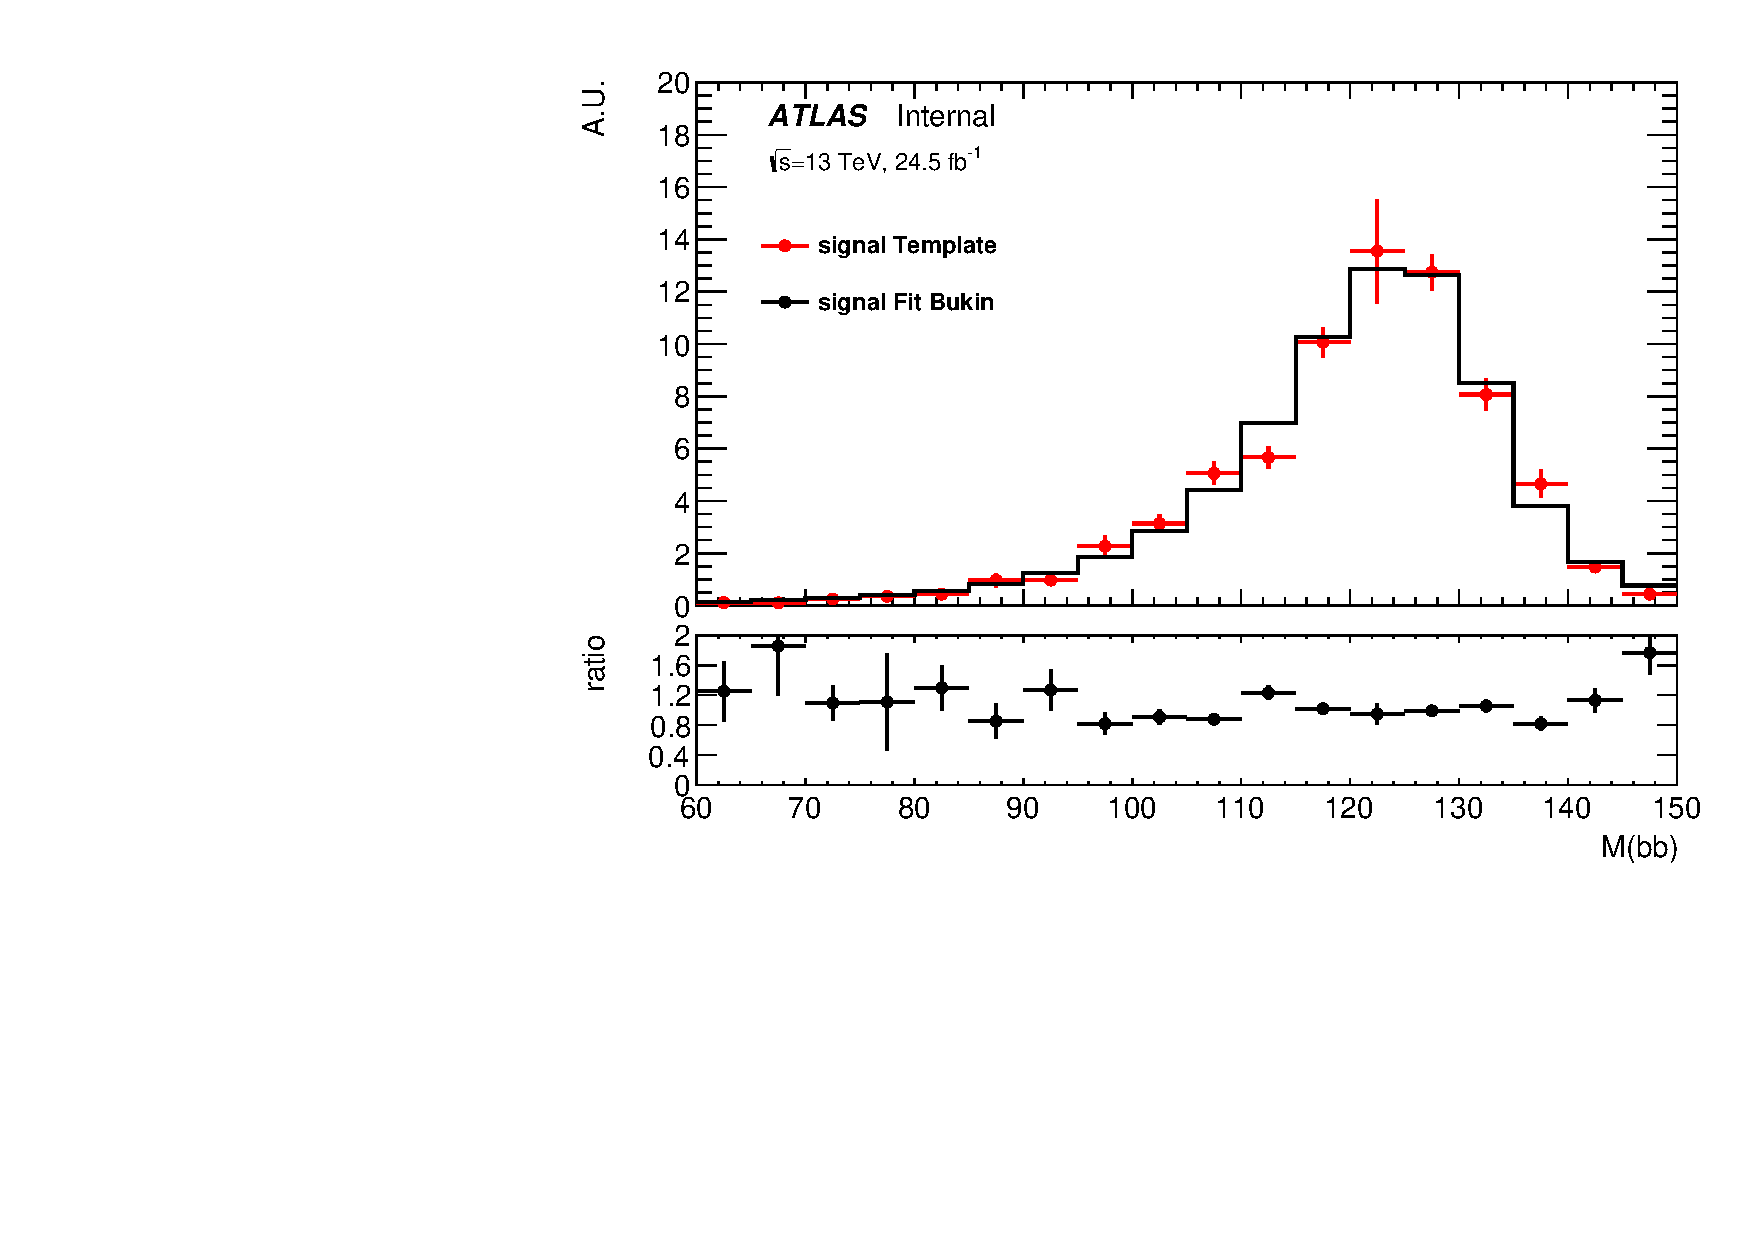
\includegraphics[width=0.45\textwidth]{figures/VBF/sig_4cen_SRI.pdf}
% 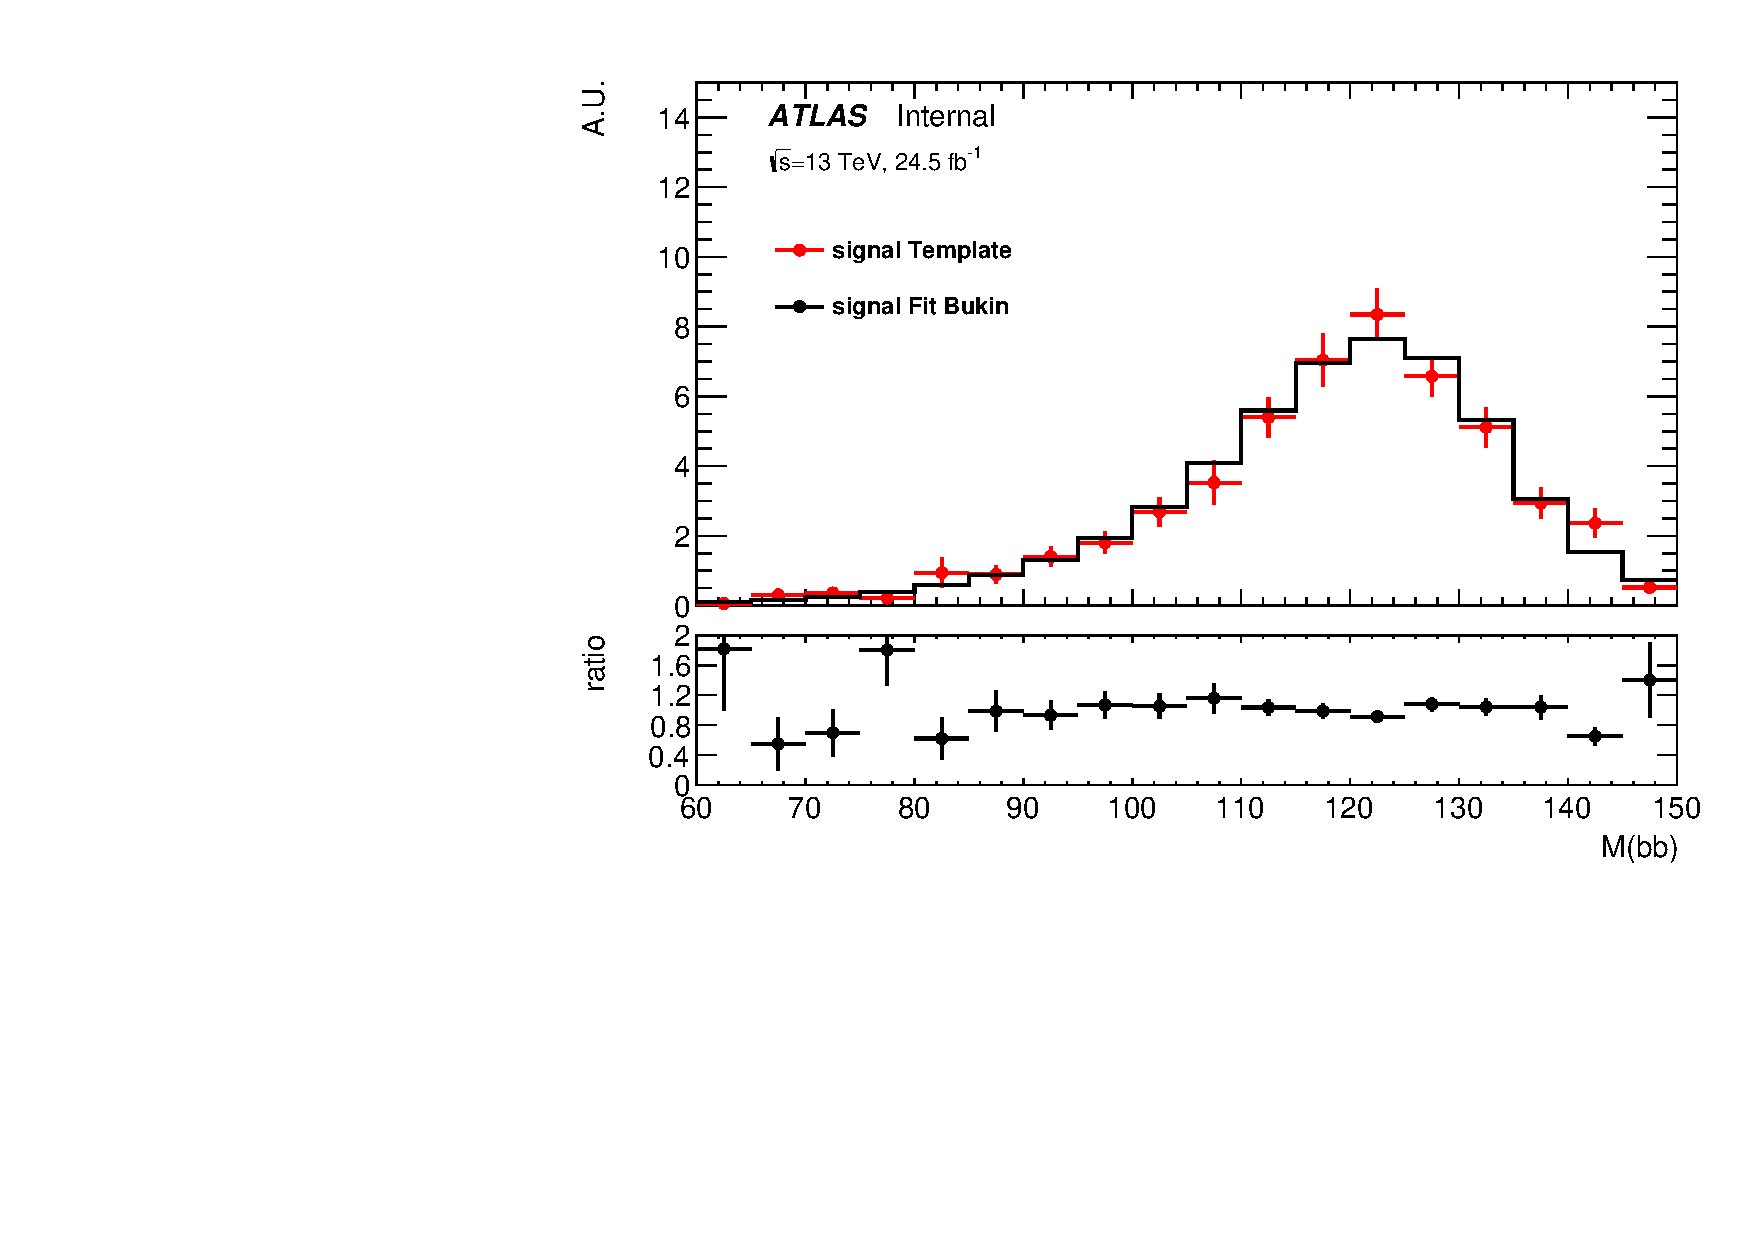
\includegraphics[width=0.24\textwidth]{figures/VBF/sig_4cen_SRII.pdf}
% 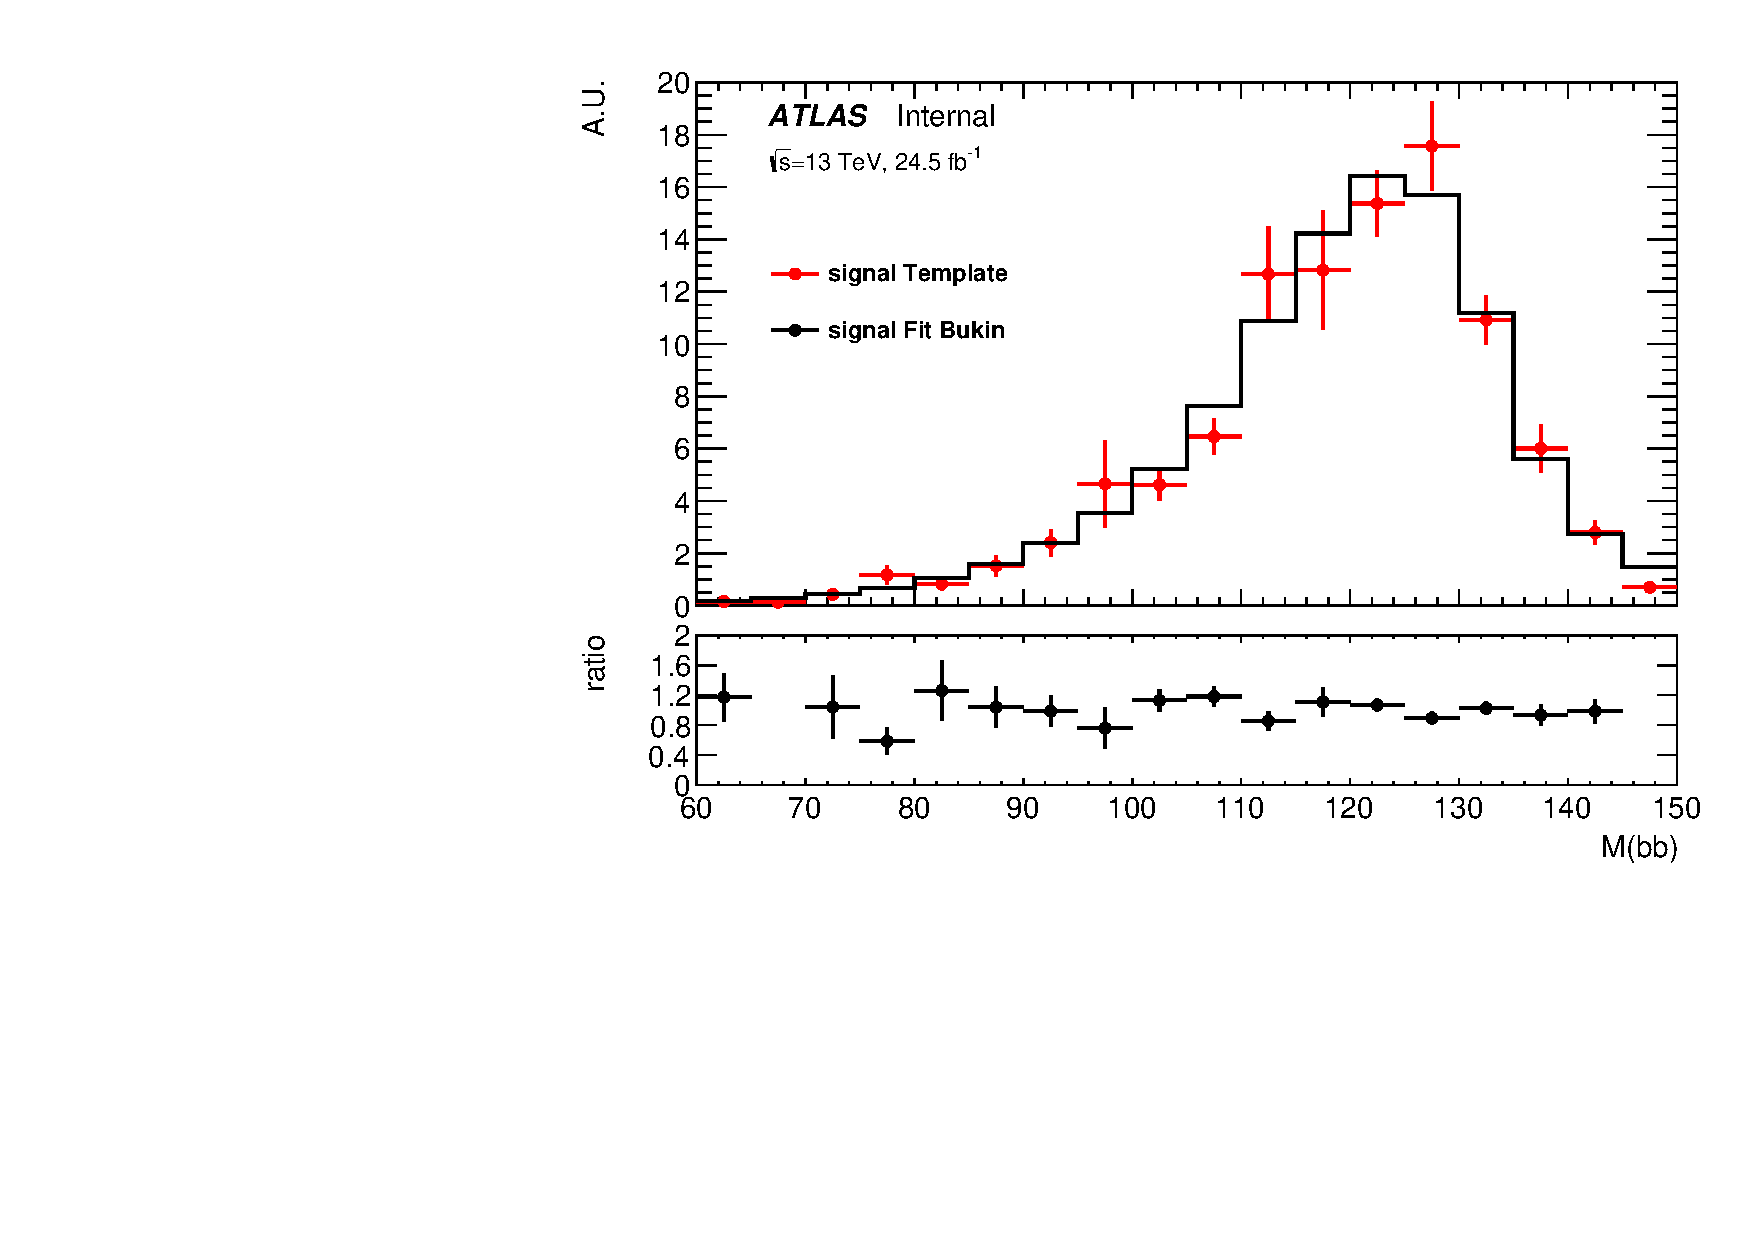
\includegraphics[width=0.24\textwidth]{figures/VBF/sig_4cen_SRIII.pdf}
% 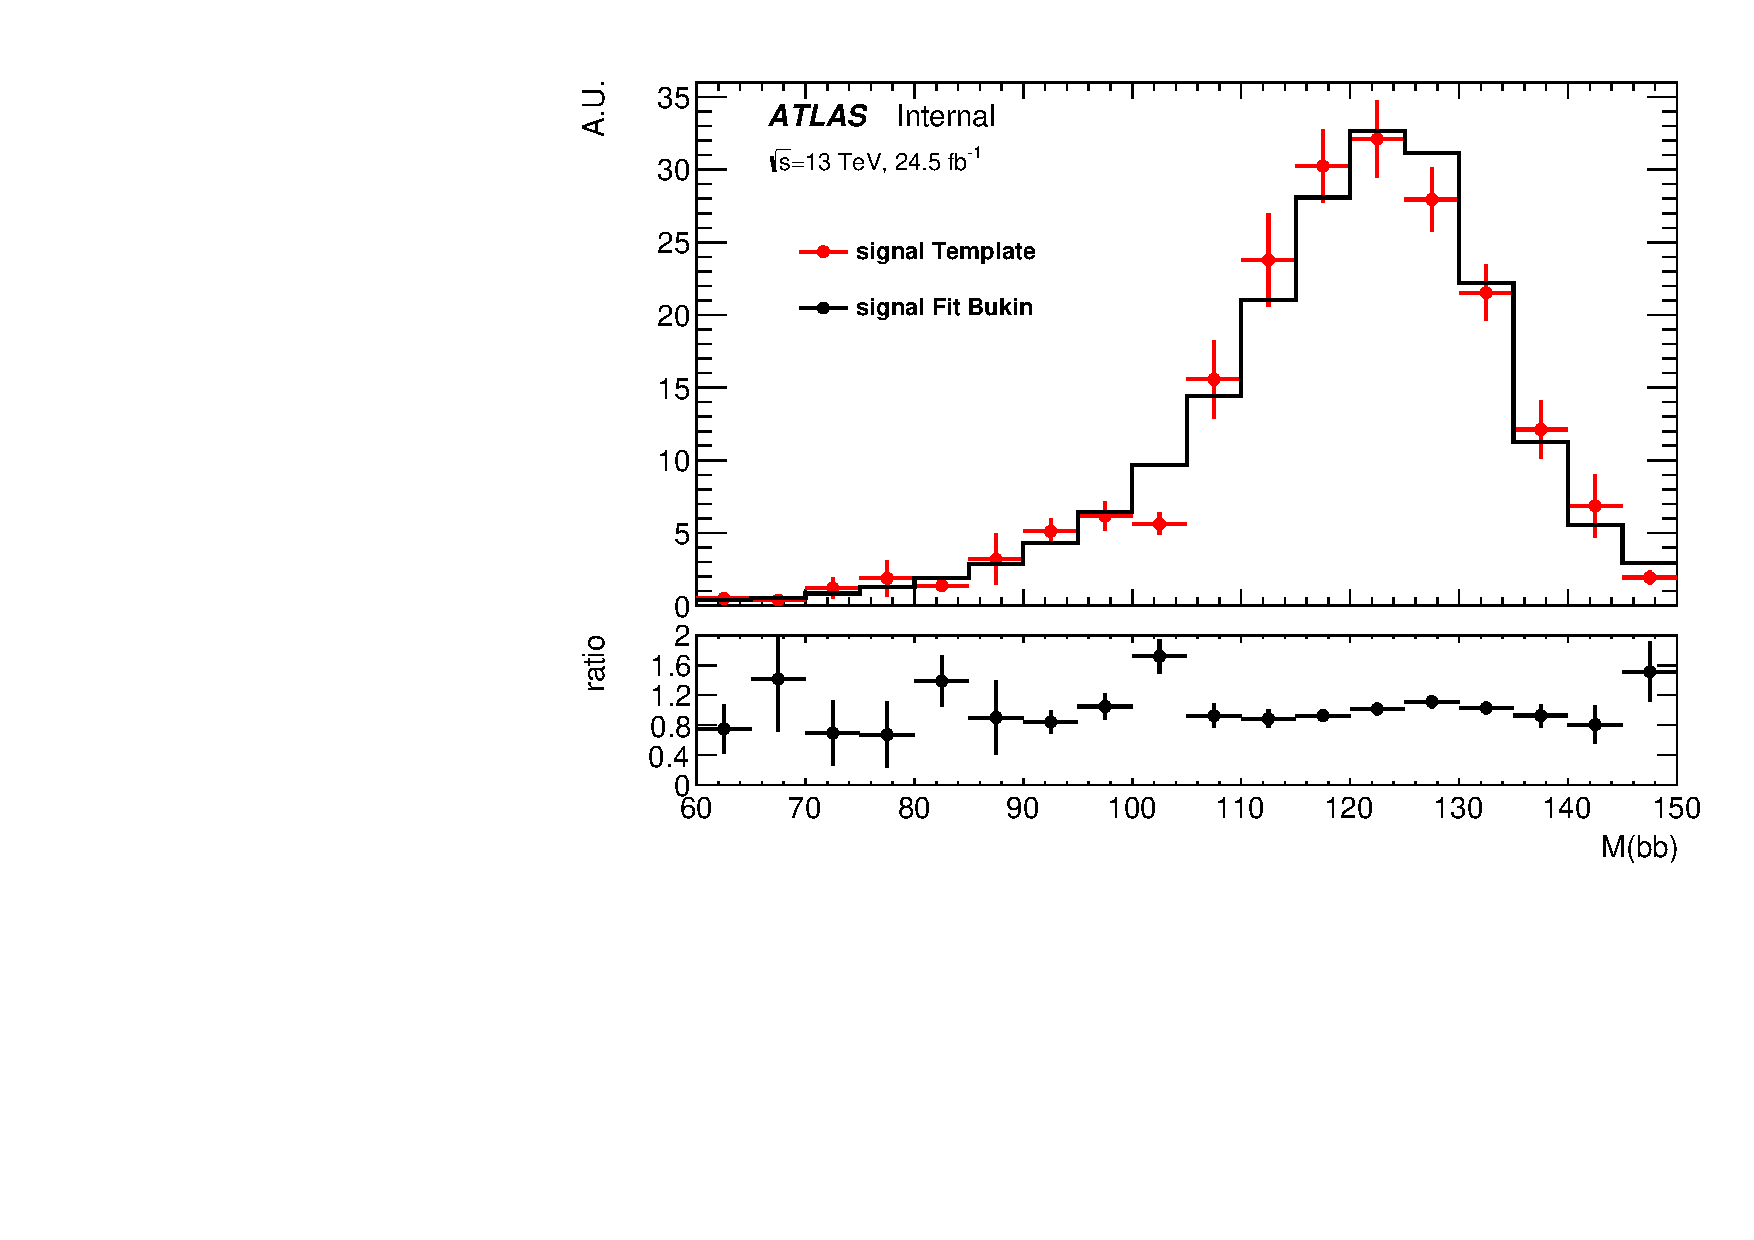
\includegraphics[width=0.24\textwidth]{figures/VBF/sig_4cen_SRIV.pdf}

\caption{Example of Bukin function parametrizations of signal \Mbb{} distributions of SR I in \twocentral channel (left) and SR I in \fourcentral channel (right)}
  \label{fig:vbf-sigpar_alt}
\end{figure}


\begin{figure}[htbp]
  \centering    
 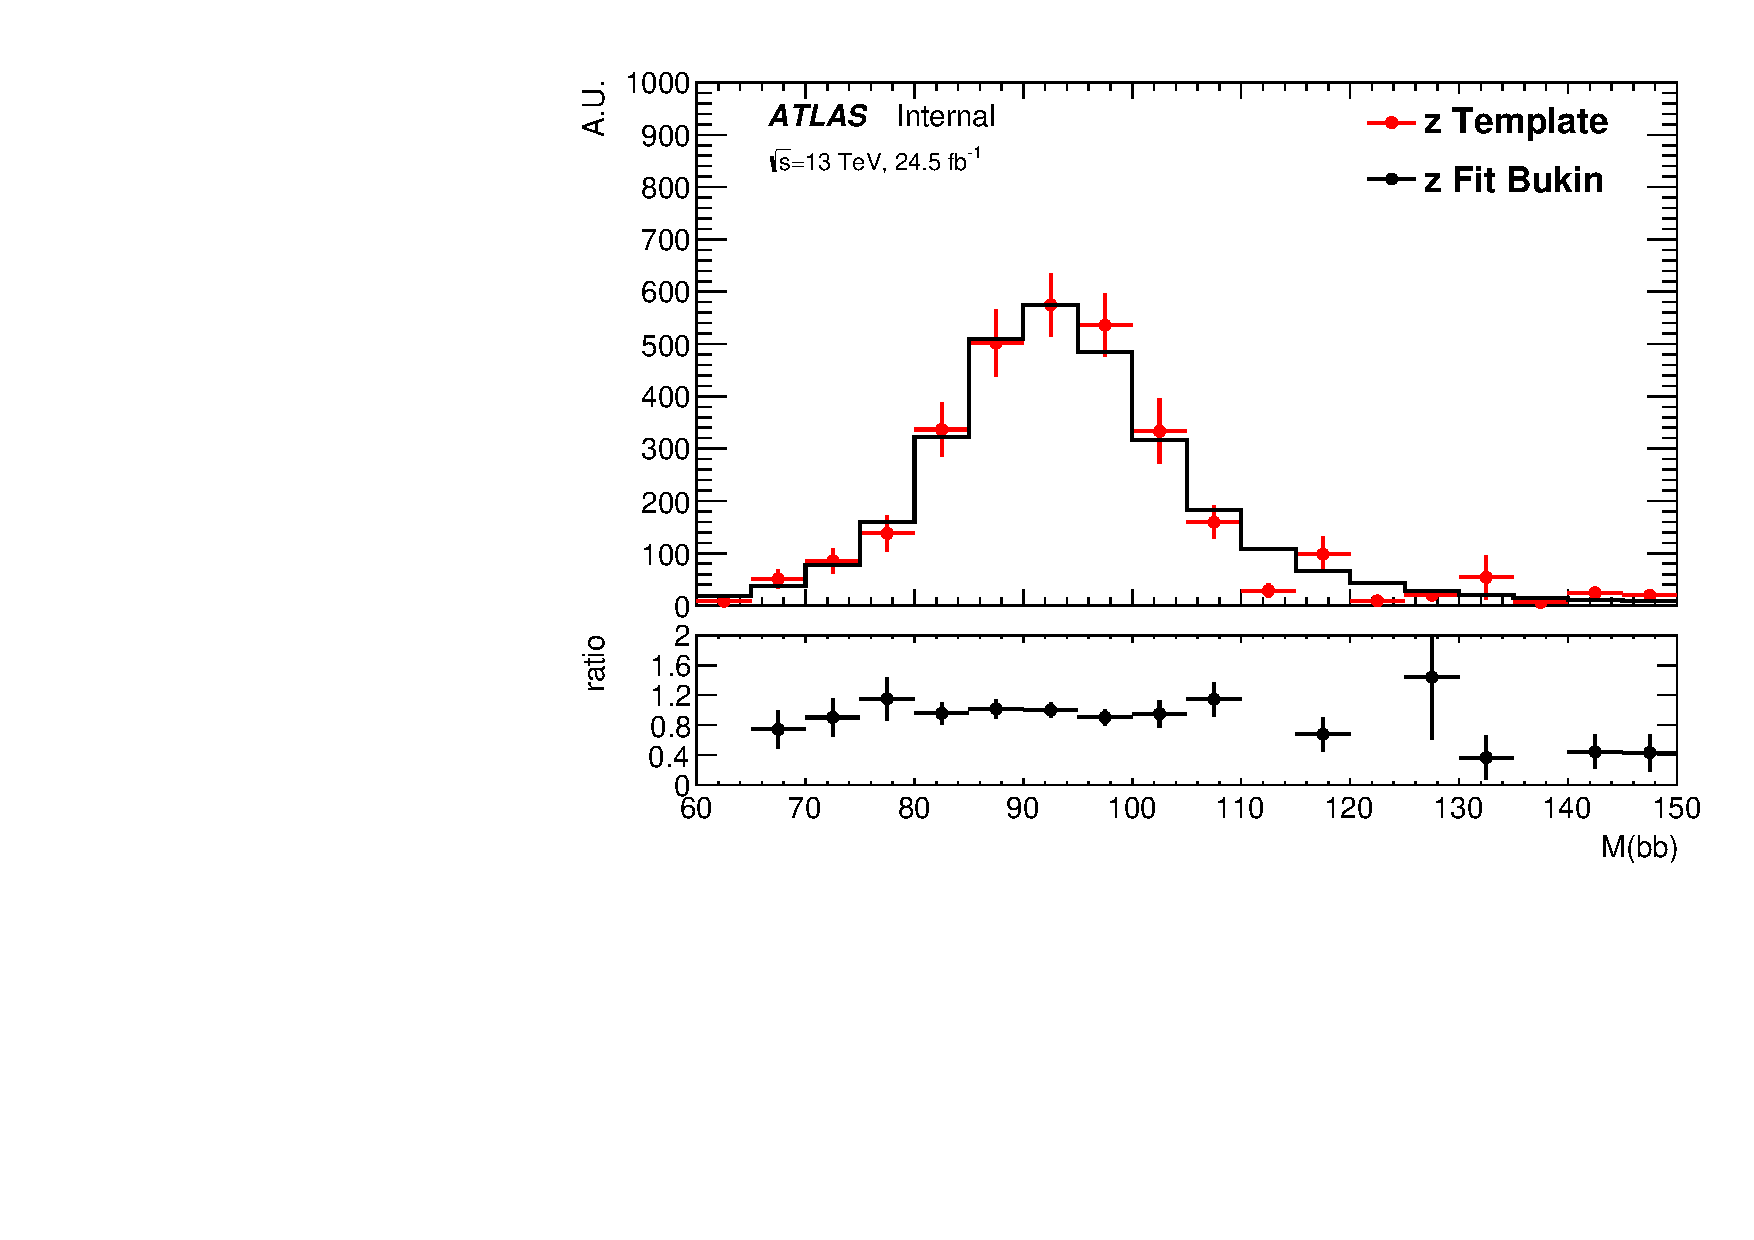
\includegraphics[width=0.45\textwidth]{figures/VBF/SigPar/z_2cen.pdf}
 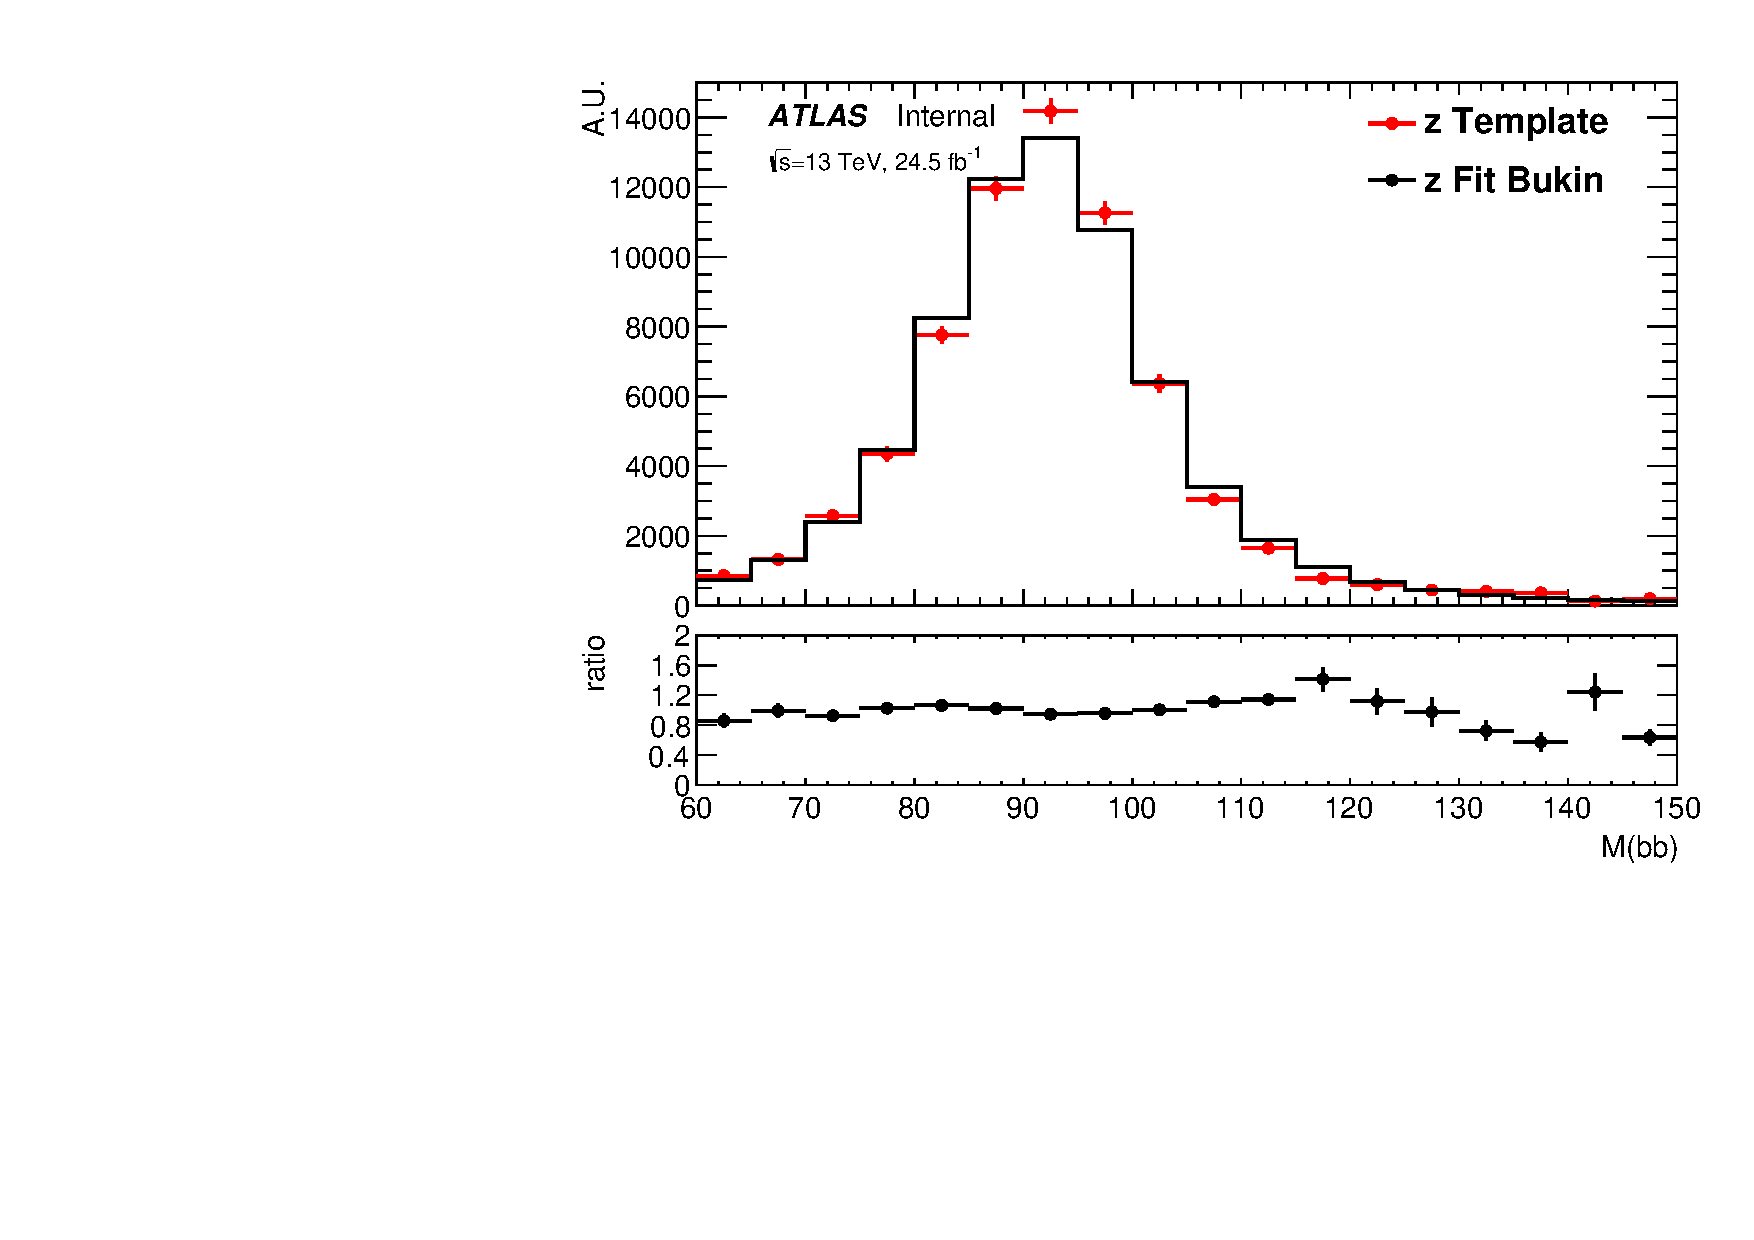
\includegraphics[width=0.45\textwidth]{figures/VBF/SigPar/z_4cen.pdf}

\caption{Bukin function parametrization of \zjets~\Mbb{} distribution in \twocentral (left) and \fourcentral (right). There are not enough events to divide the sample amongst BDT regions, therefore the distributions are shown for each channel preselection.}
\label{fig:vbf-zpar_alt}
\end{figure}


